\documentclass{article}
\usepackage{graphicx} % Required for inserting images


\title{Damped Harmonic Oscillator}
\author{Zuzana Buchová}
\date{January 2024}

\begin{document}

\maketitle

\section{Introduction}
The damped harmonic oscillator is a classical mechanical system that experiences a damping force proportional to its velocity. It is often used to model various physical phenomena, such as the motion of a mass-spring system in a viscous fluid or the behavior of electrical circuits with resistors.

\section{Basic Information}

\subsection{Equation of Motion}
The equation of motion for a damped harmonic oscillator can be expressed as:
\begin{equation}
    m\frac{\partial^2 x}{\partial t^2} + b\frac{\partial x}{\partial t} + kx = 0
\end{equation}
where:
\begin{itemize}
    \item $m$ is the mass of the oscillator
    \item $b$ is the damping coefficient (proportional to the damping force)
    \item $k$ is the spring constant
    \item $x$ is the displacement of the oscillator from its equilibrium position
    \item $t$ is time
\end{itemize}

\subsection{Damping Coefficient (\textit{b})}
The damping coefficient \textit{b} determines the strength of the damping force. It can be categorized into three regimes:
\begin{itemize}
    \item \textbf{Underdamping}($b^2 < 4mk$): Oscillations decay gradually over time.
    \item \textbf{Critical Damping}($b^2 = 4mk$): The system returns to equilibrium as quickly as possible without oscillating.
    \item \textbf{Overdamping}($b^2 > 4mk$): Oscillations are heavily damped, and the system takes a long time to return to equilibrium.
\end{itemize}

\section{Solution}
The solution to the damped harmonic oscillator equation can be written in several forms, but one common expression for the underdamped case is in terms of exponentials. The general solution is a combination of exponential functions:
\begin{equation}
    x(t) = e^{-\frac{b}{2m}t}(Acos(\omega_d t) + Bsin(\omega_d t))
\end{equation}
where:
\begin{itemize}
    \item $\omega_d = \sqrt{\omega_0^2 - (\frac{b}{2m})^2}$ is the damped angular frequency
    \item $\omega_d = \sqrt{\frac{k}{m}}$ is the natural angular frequency of the undamped oscillator
    \item  $A$ and $B$ are constants determined by initial conditions
\end{itemize}
\subsection{Particular solution}
Let's consider the underdamped case of a damped harmonic oscillator. For simplicity, let's assume $m$ = 1, $b$ = 0.5, $k$ = 4. Suppose at $t$ = 0 the displacement $x$(0) = 1. This results in an underdamped system.
Now, the solution to the underdamped harmonic oscillator equation is given by:
\begin{equation}
    x(t) = e^{-\frac{b}{2m}t}(Acos(\omega_d t) + Bsin(\omega_d t))
\end{equation}
Let's calculate the displacement at $t$ = 1.

\subsubsection{Calculate Damped Angular Frequency}
\begin{equation}
    \omega_d = \sqrt{\frac{k}{m}} = \sqrt{\frac{4}{1}} = 2
    \omega_d = \sqrt{\omega_0^2 - (\frac{b}{2m})^2} = \sqrt{2^2 - (\frac{0.5}{2})^2} = \sqrt{3.937} = 1.984
 \end{equation}
\subsubsection{Formulate the Solution}
he general solution for the underdamped harmonic oscillator is:

\begin{equation}
    x(t) = e^{-\frac{b}{2m}t}(Acos(\omega_d t) + Bsin(\omega_d t))
\end{equation}

\subsubsection{Apply Initial Conditions}
Given $x$(0)=1, we can find $A$:
\begin{equation}
    x(0) = Acos(0) + Bsin(0)
    A = 1
\end{equation}
Now, we have the specific solution:
\begin{equation}
    x(t) = e^{-0.25t}cos(1.984t)
    \end{equation}
\begin{equation}   
    x(1) = e^{-0.25}cos(1.984) = - 0.314
\end{equation}
\begin{figure}[h]
    \centering
    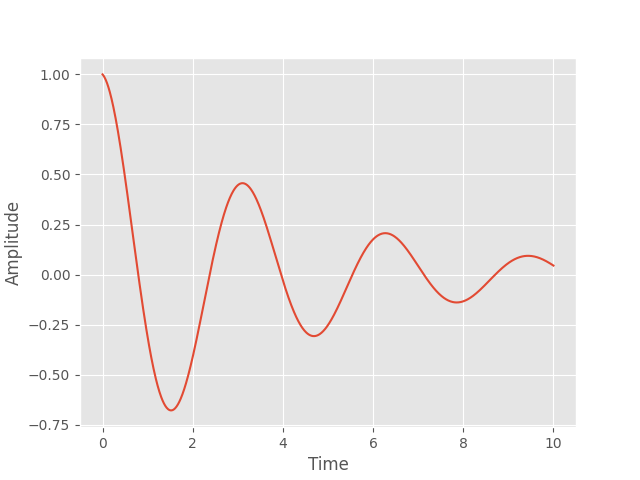
\includegraphics[width=0.7\textwidth,,keepaspectratio]{underdamped.png}
    \caption{Amplitude of underdumped oscillation as a function of time}
\end{figure}
This is the solution to the underdamped harmonic oscillator with the given initial conditions and parameters. The system will exhibit oscillatory behavior with an exponentially decaying amplitude due to the damping term. We can find the velocity ($v$) of the underdamped harmonic oscillator is given by the derivative of the displacement ($x$) with respect to time ($t$).

\end{document}
